\documentclass{article}

\usepackage{amsmath}
\usepackage{amssymb}
\usepackage{amsthm}
\usepackage{graphicx}
\usepackage{color}
\usepackage{subfig}
\usepackage{float} % For [H] placement
\usepackage{mathrsfs}   % \mathscr L_2 for curly L

\usepackage{listings}
%\usepackage{algorithm}
%\usepackage{algpseudocode}
\usepackage[ruled,vlined,linesnumbered]{algorithm2e}

\usepackage{booktabs}

\usepackage[bookmarks=true,ocgcolorlinks=true,plainpages=false, breaklinks=true, bookmarksopen=true, bookmarksnumbered=true]{hyperref}
%\usepackage[bookmarks=false]{hyperref}  %hide the bookmarks bar
%\hypersetup{bookmarksopen=false}  % expand tree of bookmarks or just show first level

\hypersetup{linkcolor=blue, citecolor=magenta,urlcolor=blue} % electronic
\hypersetup{colorlinks=true}

\usepackage{siunitx}
% \sisetup{%
%   mode = math,
% %  per-mode = symbol,
% %  per-mode=repeated-symbol,
%   per-mode=reciprocal,
%   detect-all
% }
\sisetup{per-mode=reciprocal}

\usepackage[T1]{fontenc}
\usepackage{palatino}

\allowdisplaybreaks

%%BeginIpePreamble

\newcommand{\secref}[1]{\S\ref{#1}}
\newcommand{\psubref}[1]{\protect\subref{#1}}

\renewcommand{\qedsymbol}{$\blacksquare$}
\renewcommand{\vec}[1]{\ensuremath{{\boldsymbol #1}}}
\newcommand{\mat}[1]{\ensuremath{\boldsymbol{#1}}}
\newcommand{\textscript}[1]{\textnormal{\scriptsize #1}}
\newcommand{\Tr}{\textnormal{Tr}}
\newcommand{\degrees}{\ensuremath{^\circ}}
\newcommand{\degree}{\ensuremath{^\circ}}

\newcommand{\PSF}{\textnormal{PSF}}

\newcommand{\superscript}[1]{\ensuremath{^{\textrm{#1}}}}
\renewcommand{\th}[0]{\superscript{th}}
\newcommand{\st}[0]{\superscript{st}}
\newcommand{\nd}[0]{\superscript{nd}}
\newcommand{\rd}[0]{\superscript{rd}}

\newcommand{\rect}{\ensuremath{\mathrm{rect}}}

\newcommand{\pd}[2]{\frac{\partial{#1}}{\partial{#2}}}

\DeclareMathOperator*{\argmin}{arg\,min}
\DeclareMathOperator*{\argmax}{arg\,max}
\DeclareMathOperator*{\var}{var}
\DeclareMathOperator*{\diag}{diag}
\DeclareMathOperator*{\rem}{rem}
\DeclareMathOperator*{\sign}{sgn}
\DeclareMathOperator*{\supp}{supp}
\DeclareMathOperator*{\comb}{comb}
\DeclareMathOperator*{\sinc}{sinc}
\DeclareMathOperator*{\curl}{curl}
\DeclareMathOperator*{\diverge}{div}
\DeclareMathOperator*{\image}{Im}
\DeclareMathOperator*{\rank}{rank}
\DeclareMathOperator*{\range}{range}
\DeclareMathOperator*{\Real}{Re}
\DeclareMathOperator*{\Imag}{Im}

%%EndIpePreamble


\title{PCRB}

\date{\today}

\begin{document}

\section{Model}

The model takes the form
\begin{subequations}
\begin{align}
	\vec x_k &= \vec f_k(\vec x_{k-1}) + \vec v_k \\
	\vec y_k &= \mat H\vec x_{k-1} + \vec w_k
\end{align}
\label{eqn:model_general}
\end{subequations}
where $\vec v_k$ and $\vec w_k$ are white, uncorrelated, zero mean Gaussian noise vectors with covariances of $\mat Q$ and $\mat R$, respectively. For this model the transition density is defined as
\begin{align}
	p(\vec x_k|\vec x_{k-1}) &= \mathcal N(\vec f(\vec x_{k-1})),\mat Q) \\
	&= (2\pi)^{-d/2} |\mat Q|^{-1/2} \exp\left(-\frac{1}{2}(\vec x_k - \vec f(\vec x_{k-1}))^T \mat Q^{-1} (\vec x_k - \vec f(\vec x_{k-1})) \right)
\end{align}
and the likelihood is
\begin{align}
	p(\vec y_k|\vec x_k) &= \mathcal N(\mat H\vec x_k,\mat R) \\
	&= (2\pi)^{-n/2} |\mat R|^{-1/2} \exp\left(-\frac{1}{2}(\vec y_k - \mat H\vec x_k)^T \mat R^{-1} (\vec y_k - \mat H\vec x_k) \right)
\end{align}

\section{PCRB}

The PCRB is computed from the Fisher information matrix computed on the joint density $p(\vec y,\vec x)$,
\begin{align}
	\mat J &= \mathbb E\left[ \nabla_{\vec x}\nabla_{\vec x}^T \log p(\vec y,\vec x) \right]
\end{align}
where the expectation is taken over $\vec y$ and $\vec x$. The PCRB bounds the covariance of an unbiased estimator, $\mat P$,
\begin{align}
	\mat P &\ge \mat J^{-1}
\end{align}


Recursive formulas are based on the logarithm of the likelihood and transition densities, which for the model above are
\begin{align}
	\log p(\vec x_k|\vec x_{k-1}) &= C_1 -\frac{1}{2}(\vec x_k - \vec f(\vec x_{k-1}))^T \mat Q^{-1} (\vec x_k - \vec f(\vec x_{k-1})) \\
	\log p(\vec y_k|\vec x_k) &= C_2 -\frac{1}{2}(\vec y_k - \mat H\vec x_k)^T \mat R^{-1} (\vec y_k - \mat H\vec x_k)
\end{align}

\subsection{Fisher information recursion (non-singular $Q$)} 
A recursive formula for the FIM, $\mat J_k$, was developed in \cite{Tichavsky1998}. The recursion proceeds as
\begin{align}
	\mat J_k(\vec x_k) &= \mat W_k - \mat V_k^T\left[ \mat J_{k-1}(\vec x_{k-1}) + \mat U_k\right]^{-1}\mat V_k 
\end{align}
where
\begin{align}
	\mat U_k &= -\mathbb E\left[ \nabla_{\vec x_{k-1}}\nabla_{\vec x_{k-1}}^T \log p(\vec x_k|\vec x_{k-1}) \right] \label{eqn:recursion_U}\\
	\mat V_k &= -\mathbb E\left[ \nabla_{\vec x_{k-1}}\nabla_{\vec x_k}^T \log p(\vec x_k|\vec x_{k-1}) \right] \label{eqn:recursion_V}\\
	\mat W_k &= -\mathbb E\left[ \nabla_{\vec x_k}\nabla_{\vec x_k}^T \log p(\vec x_k|\vec x_{k-1}) \right] - \mathbb E\left[ \nabla_{\vec x_k}\nabla_{\vec x_k}^T \log p(\vec y_k|\vec x_k) \right] \label{eqn:recursion_W}
\end{align}

The derivatives for the above model are
\begin{align}
	\nabla_{\vec x_k}^T \log p(\vec x_k|\vec x_{k-1}) &= -(\vec x_k - \vec f(\vec x_{k-1}))^T\mat Q^{-1}  \\
	\nabla_{\vec x_k}\nabla_{\vec x_k}^T \log p(\vec x_k|\vec x_{k-1}) &= -\mat Q^{-1} \\
	\nabla_{\vec x_{k-1}}\nabla_{\vec x_k}^T \log p(\vec x_k|\vec x_{k-1}) &= \mat F(\vec x_{k-1})\mat Q^{-1} \\
	\nabla_{\vec x_{k-1}}^T \log p(\vec x_k|\vec x_{k-1}) &= (\vec x_k - \vec f(\vec x_{k-1}))^T\mat Q^{-1} \mat F(\vec x_{k-1}) \\
	\nabla_{\vec x_{k-1}}\nabla_{\vec x_{k-1}}^T \log p(\vec x_k|\vec x_{k-1}) &= -\mat F(\vec x_{k-1})^T\mat Q^{-1} \mat F(\vec x_{k-1}) \\
	\nabla_{\vec x_k}^T \log p(\vec y_k|\vec x_k) &= (\vec y_k - \mat H\vec x_k)^T\mat R^{-1} \mat H \\
	\nabla_{\vec x_k}\nabla_{\vec x_k}^T \log p(\vec y_k|\vec x_k) &= -\mat H^T\mat R^{-1} \mat H 
\end{align}
Substituting these into \eqref{eqn:recursion_U}--\eqref{eqn:recursion_W} gives,
\begin{align}
	 \mat U_k &= \mathbb E\left[ \mat F(\vec x_{k-1})^T\mat Q^{-1} \mat F(\vec x_{k-1}) \right ] \label{eqn:pcrb_u} \\
	\mat V_k &= \mathbb E\left[ -\mat F(\vec x_{k-1})^T\mat Q^{-1} \right ] \label{eqn:pcrb_v} \\
	\mat W_k &= \mat H^T\mat R^{-1}\mat H + \mat Q^{-1}
\end{align}

When noise is only added to a subset of the states each transition, $\mat Q$ is singular and $\mat Q^{-1}$ does not exist. Another method is required.

\subsection{Cramer-Rao bound recursion (singular $Q$)} 

An alternative formulation is to recursively compute the bound at each step. That is, compute $\mat P_k = \mat J_k^{-1}$ directly rather than $\mat J_k$. The formulas suggested in \cite{Bergman2001} are applicable to wider class of models (e.g. multiplicative noise), denoted by a general transition function $\tilde{\vec f}(\vec x_k,\vec v_k)$. The recursion is
\begin{align}
	\mat P_{k|k-1} &= \bar{\mat F}_k\mat P_{k-1|k-1}\bar{\mat F}_k + \bar{\mat G}_k\mat Q_k \bar{\mat G}_k^{-1} \\
		\mat P_{k|k} &= \left(\mat P_{k|k-1}^{-1} + \bar{\mat R}_{k-1}^{-1}\right)^{-1}
\end{align}
where
\begin{align}
	\bar{\mat F}_k &= \mathbb E \left[ \nabla_{\vec x_k}^T \tilde{\vec f_k}(\vec x_k,\vec v_k)\right] \\
	\bar{\mat R}_k^{-1} &= -\mathbb E\left[ \nabla_{\vec x_k}\nabla_{\vec x_k}^T \log p(\vec y_k|\vec x_k) \right] \\
	\bar{\mat G}_k &= \mathbb E \left[ \nabla_{\vec v_k}^T \tilde{\vec f_k}(\vec x_k,\vec v_k)\right] \\
	\mat Q_k^{-1} &= -\mathbb E \left[ \nabla_{\vec v_k}\nabla_{\vec v_k}^T \log p(\vec v_k) \right]
\end{align}
and $\mat P_0^{-1}$ is the inverse of the prior covariance. The model in \eqref{eqn:model_general} is represented by $\tilde{\vec f}(\vec x_k,\vec v_k) = \vec f(\vec x_k) + \vec v_k$. This simplifies the derivatives to
\begin{align}
	\nabla_{\vec x_k}^T \tilde{\vec f_k}(\vec x_k,\vec v_k) &= \mat F_k(\vec x_k) \\
	\nabla_{\vec v_k}^T \tilde{\vec f_k}(\vec x_k,\vec v_k) &= \mat I_{d\times d} \\
	\nabla_{\vec x_k}\nabla_{\vec x_k}^T \log p(\vec y_k|\vec x_k) &= -\mat H^T\mat R^{-1} \mat H 
\end{align}
and the corresponding matrices to	
\begin{align}
	\bar{\mat F}_k &= \mathbb E\left[ \mat F_k(\vec x_k)\right] \label{eqn:pcrb_term_F}\\
	\bar{\mat R}_k^{-1} &= \mat H^T\mat R^{-1} \mat H \\
	\bar{\mat G}_k &= \mat I_{d\times d} 
\end{align}
Notice that $\mat Q^{-1}$ is not directly required in the recursion, so this method is applicable to neural field models where process noise is only added to a single state.

\subsection{Monte Carlo approximations}

The expectations in \eqref{eqn:pcrb_u} and \eqref{eqn:pcrb_v} or \eqref{eqn:pcrb_term_F} can be approximated by numerical integration using many trajectory realisations. That is,
\begin{align}
	\mat U_k &\approx \frac{1}{M}\sum_{i=1}^M \mat F(\vec x_{k-1}^{(i)})^T\mat Q^{-1} \mat F(\vec x_{k-1}^{(i)}) \\
	\mat V_k &\approx \frac{1}{M}\sum_{i=1}^M \mat F(\vec x_{k-1}^{(i)})^T\mat Q^{-1}  
\end{align}
or alternatively,
\begin{align}
	\bar{\mat F}_{k-1} &\approx \frac{1}{M}\sum_{i=1}^M \mat F(\vec x_{k-1}^{(i)})
\end{align}

\subsection{Analytical evaluation of expectations}

For the JR model the expectation in \eqref{eqn:pcrb_term_F} above is
\begin{align}
	\bar{\mat F}_k &= \mathbb E\left[ \mat F_k(\vec x_k)\right] \\
	&= \mat F_k^{\rm (lin)} + \mathbb E\left[ \mat G_k(\vec x_k)\right] 
\end{align}
where $\mat G_k(\vec x_k)$ contains the nonlinear component of the Jacobian, i.e., terms such as
\begin{align}
	\exp(-(x-v_0)^2/\zeta^2)
\end{align}
whose expectation can be evaluated as follows...


\section{Pendulum example}

Let $\vec x_k = [a_k\quad b_k]^T$ where $a_k$ is the pendulum angle and $b_k$ is the angular velocity,
\begin{align}
	\vec f(\vec x_{k}) &= \left[\begin{array}{c}
								a_k + b_k\Delta \\ -b_k - g\sin(a_k)\Delta
								\end{array}\right]
\end{align}
The linearisation used for the EKF is
\begin{align}
	\mat F(\vec x_{k}) &= \left[\begin{array}{cc}
					1 & \Delta \\
					-g\cos(a_k) & 1 \\
				\end{array}\right]
\end{align}
The observation matrix is $H=[1\quad 0]$, so that only the first state element is measured.

\subsection{Simulations}

\begin{figure}[H]
	\centering
	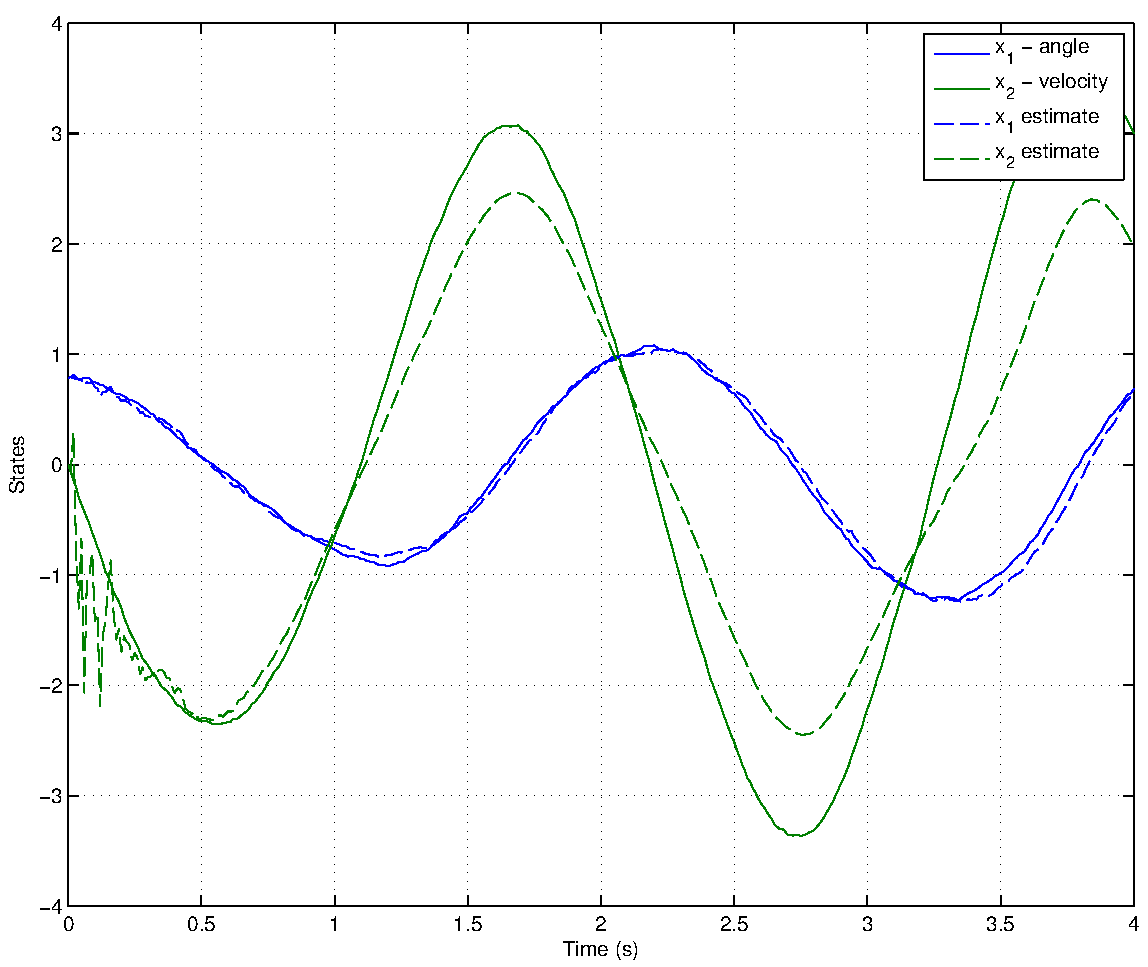
\includegraphics[width=0.75\textwidth]{../figures/pendulum_trajectory}
	\caption{Trajectory of a pendulum and EKF estimates}
\end{figure}
\begin{figure}[H]
	\centering
	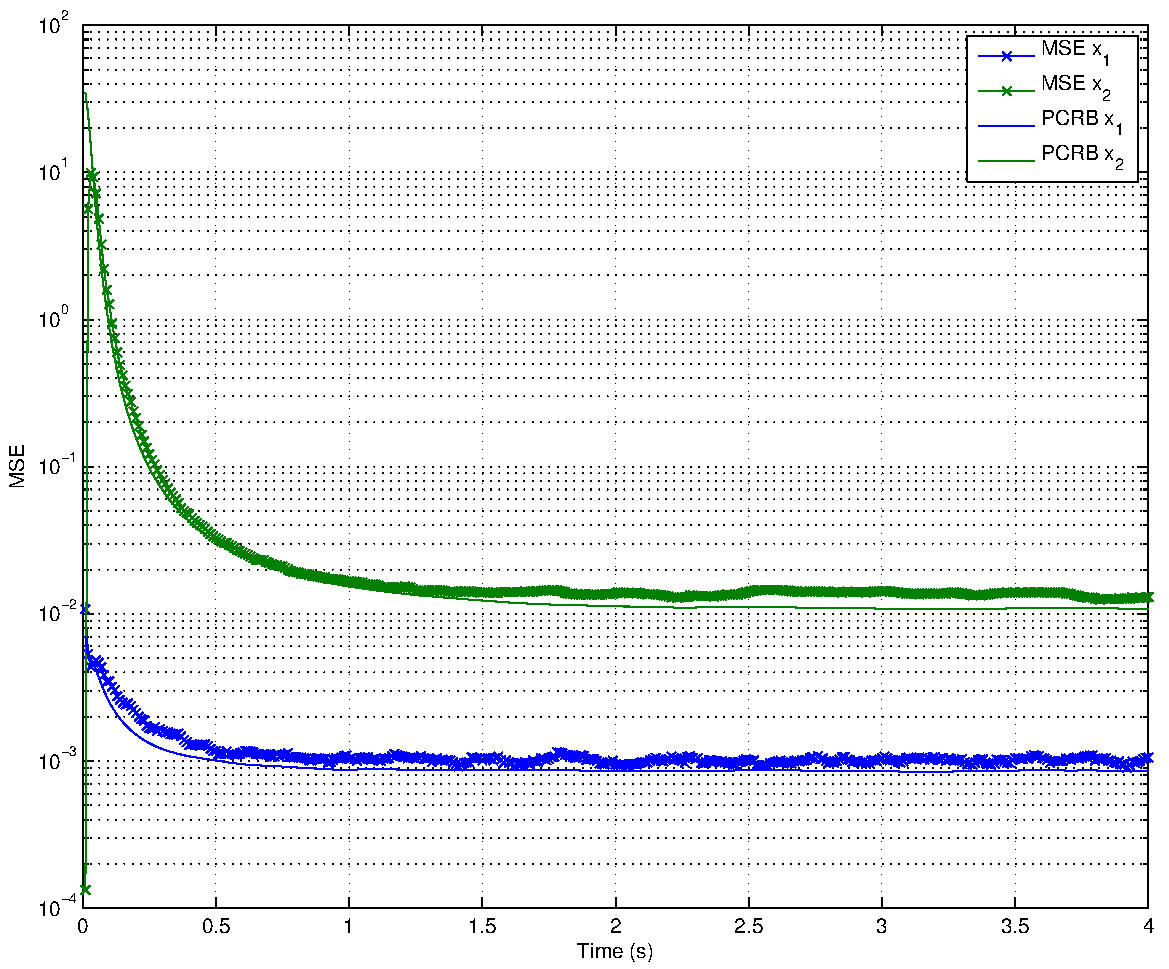
\includegraphics[width=0.75\textwidth]{../figures/pendulum_pcrb}
	\caption{MSE of EKF estimates (averaged over 1000 realisations) compared to the PCRB. The suboptimal EKF is slightly above the PCRB.}
\end{figure}

\small
\bibliographystyle{ieeetr}
\bibliography{references}
% \bibliography{../../library}



\end{document}
